\documentclass[../EDF Master Thesis.tex]{subfiles}

\begin{document}

Als Plattform für dieses Projekt dient ein STM32F769I-Disc0 Board der Firma ST.
Dieses ist mit einen ARM®Cortex®-M7 Prozessor ausgestattet und hat für die verwendete Arbeit mehr als ausreichende Rechenleistung.
Für die Kommunikation zwischen Host-Computer und Mikrocontroller wurde die integrierte Ethernet Schnittstelle verwendet.
Des Weiteren wurde eine 'Debug-Flag' integriert, welche über den integrierten \ac{usart} Debug Informationen sendet.
Dieses Flag sollte allerdings nicht im Produktivbetrieb benutzt werden, da dies zu unvorhersehbaren Verzögerungen der Tasks und im Scheduling führen kann.
Für die 'Blinky-Demo' wurden außerdem die drei, auf dem Board integrierten, \ac{led}s verwendet.

\begin{figure}[ht!]
    \begin{center}
        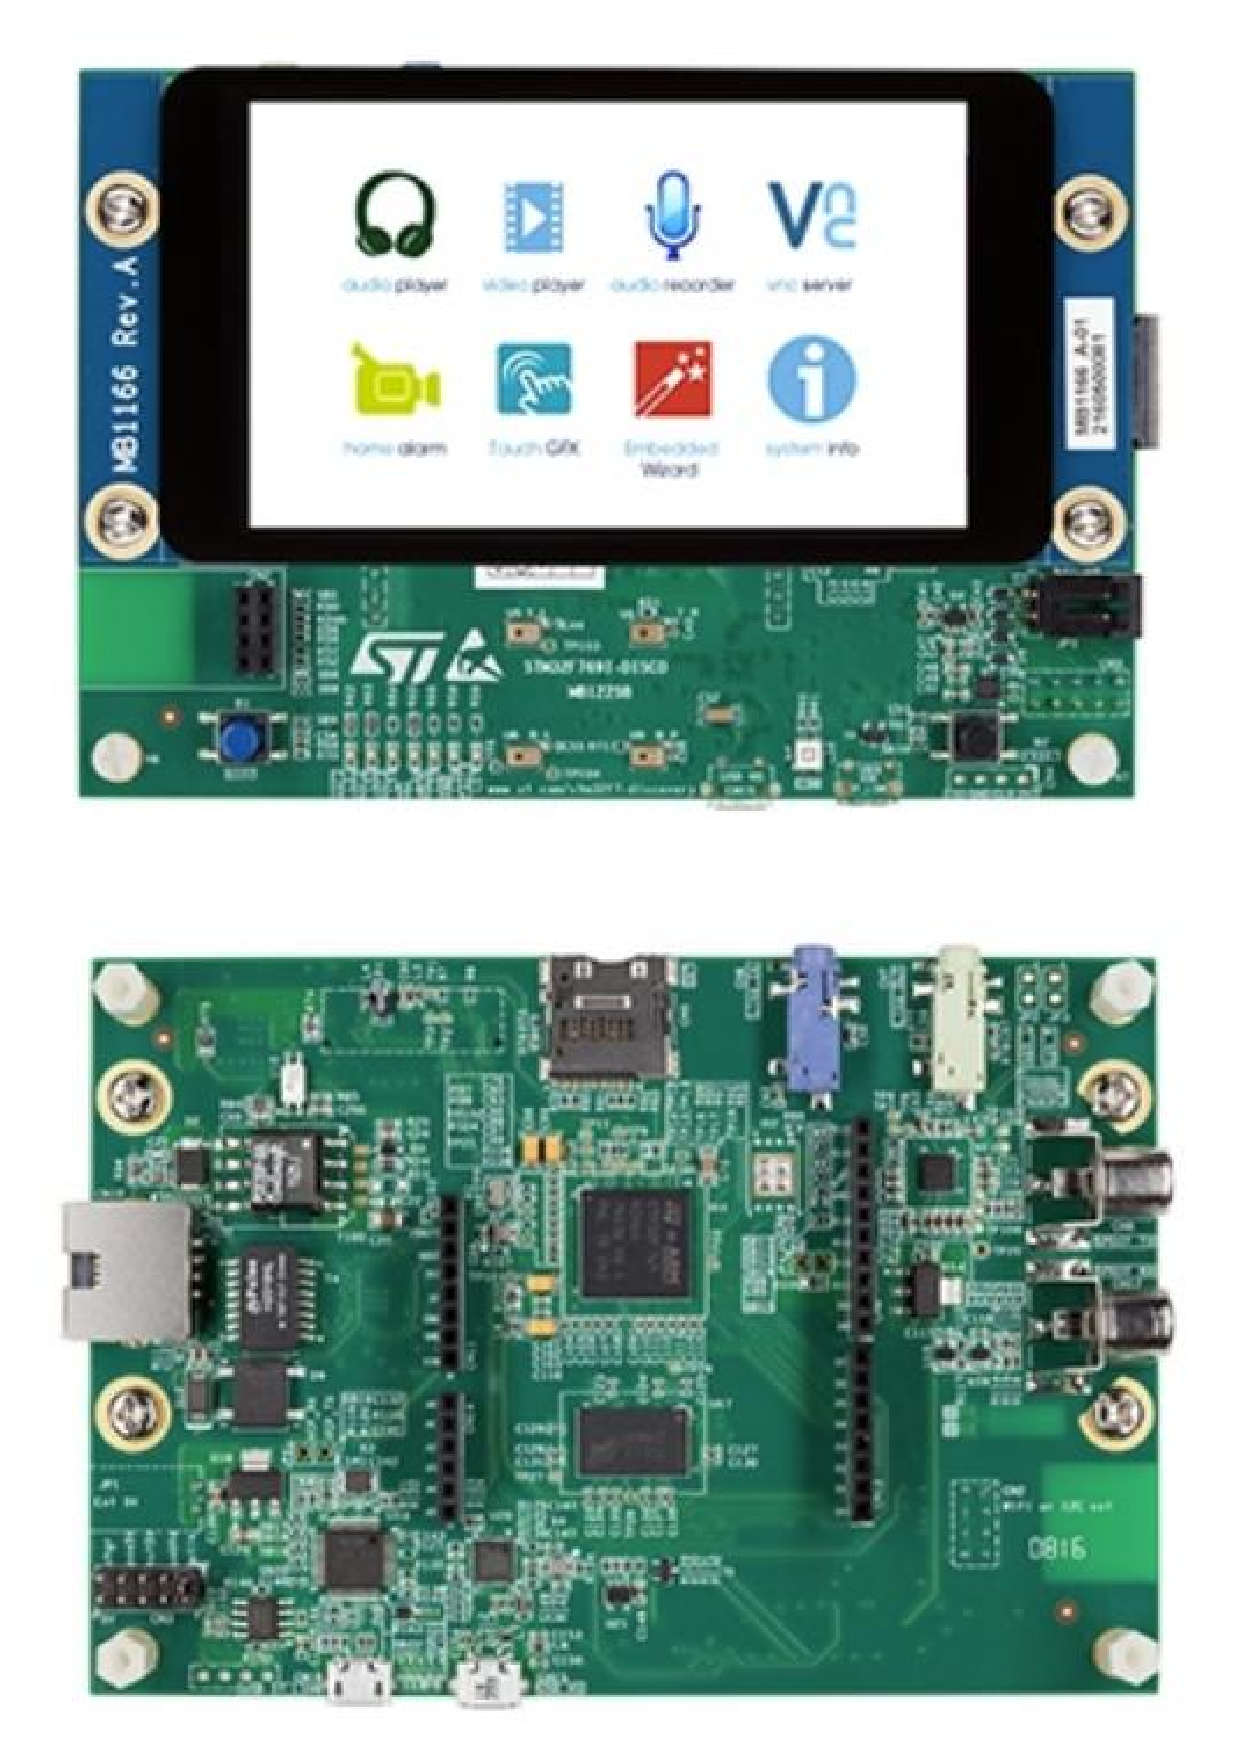
\includegraphics[width=0.6\textwidth]{attachments/stm32f769i-disc0.pdf}
    \end{center}
    \caption{STM32F769I-Disc0 Board, Quelle: \autocite{stm:001}}
    \label{fig:STM32F769I-Disc0_board}
\end{figure}

\end{document}
